\section{Parallel Implementations on CPU and GPU}
\frame{\tableofcontents[currentsection]}

\frame{ \frametitle{Introduction}
\begin{itemize}
\item ALM speeds up $\ell_1$ minimization, but still not enough!
\item This section presents parallelized implementations of the face pipeline
\item There is ample parallelism available in the pipeline
\item Leverage the high levels of concurrency available in multi-core CPU and GPU architectures.
\end{itemize}
}

\frame{ \frametitle{CPU vs. GPU architecture comparison}
\begin{itemize}
\item CPU: Intel E5530, Dual-socket, quad-core Xeon
\item GPU: Nvidia GTX480 Single-socket GPU on PCIe card
\end{itemize}

\centering
\begin{tabular}{l|c|c}
Attribute & CPU & GPU \\
\hline
Cache Size & {\color{red} 8MB} & 768 KB \\
Clock & {\color{red} 2.4 GHz} & 1.4 GHz \\
DRAM Bandwidth & 25 GB/s & {\color{red} 177 GB/s} \\
Vector Width & 4 & {\color{red} 64} \\
Cores	& 8 & {\color{red} 15} 
\end{tabular} 

\begin{itemize}
\item CPU has two levels of concurrency: {\em core-level} and {\em SSE-level}
\item GPU has two levels of concurrency: {\em SM-level} and {\em thread-level} 
\end{itemize}
}

\newcommand{\tempscale}[0]{0.8}
\frame{ \frametitle{CPU and GPU cache comparison}
\centering
The larger algorithm data structures: \\
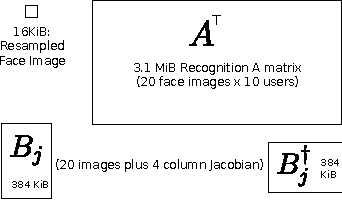
\includegraphics[scale=\tempscale]{../figures_ijcb/arrays.pdf} \\
The caches on a E5530 CPU: \\
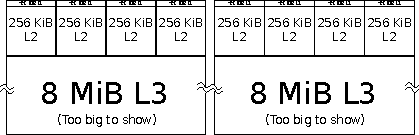
\includegraphics[scale=\tempscale]{../figures_ijcb/cpu_caches.pdf} \\
The caches on a GTX480 GPU: \\
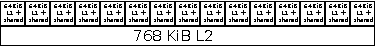
\includegraphics[scale=\tempscale]{../figures_ijcb/gpu_caches.pdf} \\
}

%\frame{ \frametitle{Limitations of CUDA programming model}
%}

\frame{ \frametitle{Parallelization of SRC recognition stage}
\begin{itemize}
\item Single large $\ell_1$ minimization problem
\item Only one level of parallelism available: {\em pixel-level}
\item Essentially one essential parallelization strategy:\\
Map pixel-level parallelism onto both core-level and vector-level concurrency
\item Leverage built-in parallelization of MKL BLAS  and CUBLAS libraries
\item Array storage implicitly affects parallelization within the BLAS implementation
\end{itemize}
}
%\frame{ \frametitle{Parallelization of SRC Recognition Stage}
%\begin{itemize}
%\item Most operations map directly onto calls in the BLAS API.
%\item On the CPU, Intel's MKL BLAS can exploit both levels of concurrency on the CPU.
%\item On the GPU, Nvidia's CUBLAS exploits both levels of concurrency on the CPU.
%\item On the CPU, the remaining operations can be parallelized via manual threading (via OpenMP),
%and automatic vectorization (via the Intel ICC compiler).
%\item On the GPU, the remaining operations can be parallelized manually as CUDA kernels.
%\end{itemize}
%}


\frame{ \frametitle{Effect of cache size for solving a single minimization problem}
Benchmark the generic basis pursuit problem (alternate SRC formulation):
\begin{equation} 
\min \|\xx\|_1\quad \mbox{ subj. to }\quad \bb = A\xx
\end{equation}
{ \tiny
{\bf INPUT:} $\bb \in \Re^m$, $A=[A_1,\cdots, A_K] \in \Re^{m \times n}$, $\tau\leftarrow \max\mbox{eig}(A^TA)$, and constant $\rho>1$.
\begin{algorithmic}[1]
\WHILE{not converged ($k = 1,2,\ldots$)} 
\STATE $t_1 \leftarrow 1$, $\zz_1 \leftarrow \xx_k$, $\uu_1 \leftarrow \xx_k$ 
\WHILE{not converged ($l = 1,2,\ldots$)} 
\STATE $\uu_{l+1}  \leftarrow \shrink(\zz_l - \frac{1}{\tau}A^T(A\zz_l - \bb - \frac{1}{\mu_k}\blambda_k), \frac{1}{\mu_k\tau})$
\STATE $t_{l+1} \leftarrow \frac{1}{2}( 1 + \sqrt{1+4t_l^2})$
\STATE $\zz_{l+1} \leftarrow \uu_{l+1}+ \frac{t_l - 1}{t_{l+1}}(\uu_{l+1} - \uu_l)$ 
\ENDWHILE 
\STATE $\xx_{k+1} \leftarrow \uu_{l+1}$ 
\STATE $\blambda_{k+1} \leftarrow \blambda_k + \mu_k (\bb - A\xx_{k+1})$ 
\STATE $\mu_{k+1} \leftarrow \rho\cdot\mu_k$ 
\ENDWHILE 
\end{algorithmic}
{\bf OUTPUT:} $\xx^* \leftarrow \xx_k$.
}
}

\frame{ \frametitle{Effect of cache size for solving a single minimization problem}
%How does the speed of solving a single ALM problem at a time vary with problem size?
{
\tiny
\begin{itemize}
\item Random Gaussian $A \in \Re^{m \times 2*m}$, with normalized columns
\item Ground truth $\x_0$ also random Gaussian, 10\% sparsity, normalized to unit norm
\item Measurement vector $\bb = A \x_0$.   
\item Termination when $\|\bx-\bx_0\| < \tau$ with $\tau=10^{-3}$.  
\item Running with single socket (4 cores, 8MB L3 cache).
\end{itemize}
}
\begin{center}
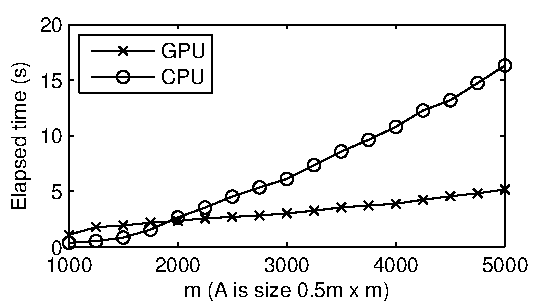
\includegraphics[width=3.5in]{../figures_ijcb/time_vs_matrix_size_constant_tol.pdf}
\end{center} 
Crossover point occurs exactly where A reaches 8MB L3 cache size!
}

\frame{ \frametitle{ALM recognition stage benchmark}
Recognition stage runtime vs. face window resolution
Benchmark ALM based Recognition stage running on real data:
Images of 10 users from Iterative Alignment Stage, running on Multi-PIE.
Vary image size: $32\times32$, $48 \times 48$, $64 \times 64$, $96 \times
96$, and $128 \times 128$.  
\centering
{
	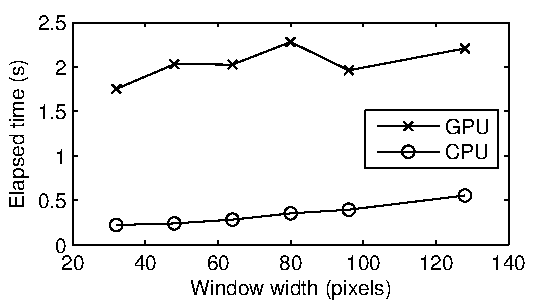
\includegraphics[width=3in]{../figures_ijcb/speedVsResolution.pdf} 
}
\begin{itemize}
\item Problem size too small to run efficiently on GPU.
\item Runtime for both implementations low compared to alignment stage.
\end{itemize}
}

\frame{ \frametitle{Parallelization of iterative alignment}
\begin{itemize}
\item Need to repeatedly solve many small $\ell_1$-minimization problems 
\item $\ell_1$ minimization is interleaved with image rewarping
\item Two levels of parallelism: \emph{problem-level} and \emph{pixel-level}
\end{itemize}
We consider two parallelizations of iterative alignment:
\begin{enumerate}
\item Alignment problems solved sequentially \\
\begin{itemize} 
\item problem-level parallelism unused
\item pixel-level parallelism mapped onto both vector-level and core-level hardware concurrency
\end{itemize}
\item Alignment problems solved concurrently \\
\begin{itemize} 
\item problem-level parallelism mapped onto core-level concurrency
\item pixel-level parallelism mapped onto vector-level concurrency
\end{itemize}
\end{enumerate}
}

\frame{ \frametitle{Parallelization of iterative alignment}
\begin{itemize}
\item Measure the impact of solving many $\ell_1$ problems
concurrently on the GPU
\item Benchmark three implementations of the alignment $\ell_1$-minimization solver
\item $A$ is size $5120 \times 32$
\item $50$ inner loop iterations for each of $50$ outer loop iterations. 
\item measured on GTX480 GPU 
\item The proposed parallelization of the $\ell_1$-minimization used in the alignment
stage is {\em eight times} faster than an implementation solving a single
problem at a time using the stock BLAS libraries.
\end{itemize}
\centerline{
\small
\begin{tabular}{|l|c|}
\hline
Sequential solver using CUBLAS & 302\,ms \\
\hline
One problem per SM using CUDA streams & 70\,ms  \\
\hline
Four problems per SM using single kernel & {\bf 36\,ms} \\
\hline
\end{tabular} 
}
}

\frame{ \frametitle{Parallelized alignment stage benchmark}
{
	\tiny
	\begin{itemize}
	\item CMU Multi-PIE Face Database with 249 users
	\item Gallery: Frontal images from session 1, 20 images per subject
	\item Test set: Frontal images from session 2 
	\item Alignment is performed using a $64 \times 64$ window
	\item similarity transformations with manual initialization 
	\end{itemize}
}
\centering
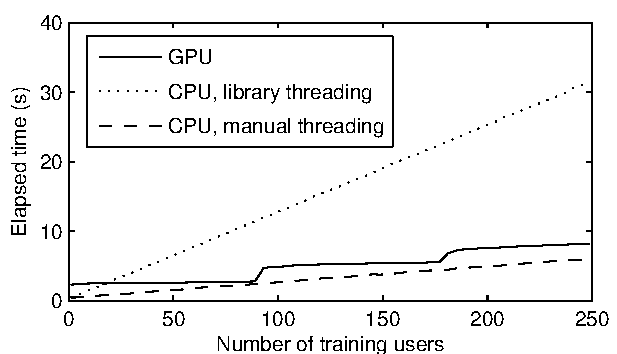
\includegraphics[width=3in]{../figures_ijcb/alignment_runtime_graph.pdf}
\begin{itemize}
\item Number of gallery subjects is varied to show scalability
\item {\em Much} faster than earlier results!
\item Recognition against 249 users in under 10s!
\end{itemize}
}

\frame{ \frametitle{Parallelized pipeline accuracy}
\centering
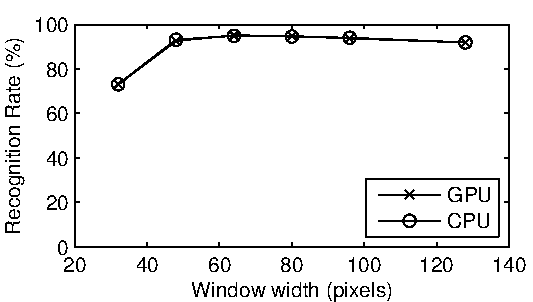
\includegraphics[width=3in]{../figures_ijcb/accuracyVsResolution.pdf} 
\begin{itemize}
\item Varied resolution of image resolution for recognition stage.
\item At the optimal resolution, the GPU implementation reaches 95\% recognition rate, the max
achievable given the selected recognition users.  
\item For significantly lower resolutions, the accuracy drops off significantly.  
\item The slight difference in CPU vs. GPU accuracy may be a result of numerical precision differences in matrix
inversion and vector reduction.
\end{itemize}
}

\frame{ \frametitle{Parallelization Conclusion}
\begin{itemize}
\item For alignment stage, parallelizations of ALM that solve multiple problems concurrently are significantly
faster than implementations than naive parallel BLAS based implementations.
\item Achieved near real-time recognition performance on 8-core workstation
\item SM-level CUDA BLAS routines were painful to develop, but provide a foundation
for new $\ell_1$ solvers already under development.
\end{itemize}
Promising Future
\begin{itemize}
\item CPUs are increasing number of cores (already 12+) and vector widths (doubles with AVX)
\item GPU are increasing in amount of cache
\item $\Rightarrow$ Both architectures converging towards an architectural balance
that is more conducive to face recognition.
\item AMD APU and Intel Knight's corner architectures are attempting to blend the best
aspects of CPU and GPU.
\end{itemize}
}

